\documentclass[xcolor=x11names,compress]{beamer}

%% General document %%%%%%%%%%%%%%%%%%%%%%%%%%%%%%%%%%
\usepackage{graphicx}
\usepackage{color}
\usepackage{tikz}
\usepackage{endnotes}
\usepackage{tikz-qtree}
\usetikzlibrary{decorations.fractals}
\usetikzlibrary{shapes,arrows}
%%%%%%%%%%%%%%%%%%%%%%%%%%%%%%%%%%%%%%%%%%%%%%%%%%%%%%


%% Beamer Layout %%%%%%%%%%%%%%%%%%%%%%%%%%%%%%%%%%
\useoutertheme[subsection=false,shadow]{miniframes}
\useinnertheme{default}
\usefonttheme{serif}
\usepackage{palatino}

\setbeamerfont{title like}{shape=\scshape}
\setbeamerfont{frametitle}{shape=\scshape}

\definecolor{PSUgrey}{HTML}{76794e}
\definecolor{PSUblue}{HTML}{00719d}
\definecolor{PSUdarkgreen}{HTML}{5e8125}
\definecolor{PSUlightgreen}{HTML}{a7b52a}

\setbeamercolor*{lower separation line head}{bg=PSUdarkgreen} 
\setbeamercolor*{normal text}{fg=white!50,bg=black} 
\setbeamercolor*{alerted text}{fg=PSUblue} 
\setbeamercolor*{example text}{fg=PSUgrey} 
\setbeamercolor*{structure}{fg=PSUlightgreen} 
 
\setbeamercolor*{palette tertiary}{fg=PSUdarkgreen,bg=black!80} 
\setbeamercolor*{palette quaternary}{fg=PSUdarkgreen,bg=black!80} 

\setbeamerfont{block title}{size=\scriptsize}
\setbeamerfont{block body}{size=\scriptsize}

\hypersetup{colorlinks,linkcolor=PSUgrey,urlcolor=PSUgrey}

% Define block styles
\tikzstyle{decision} = [diamond, draw, fill=blue!20, 
    text width=4.5em, text badly centered, node distance=3cm, inner sep=0pt]
\tikzstyle{block} = [rectangle, draw, fill=PSUblue, 
    text centered, rounded corners, minimum height=2em]
\tikzstyle{line} = [draw, -latex']
\tikzstyle{cloud} = [draw, ellipse,fill=PSUdarkgreen, node distance=3cm,
    minimum height=2em]

\renewcommand{\(}{\begin{columns}}
\renewcommand{\)}{\end{columns}}
\newcommand{\<}[1]{\begin{column}{#1}}
\renewcommand{\>}{\end{column}}

\newenvironment<>{asideblock}[1]{%
	\begin{actionenv}#2%
		\def\insertblocktitle{#1}%
		\par%
		\mode<presentation>{%
			\setbeamercolor{block title}{fg=white,bg=PSUblue}
			\setbeamercolor{block body}{fg=white,bg=black!80}
			\setbeamertemplate{blocks}[rounded][shadow=true]
		}%
		\usebeamertemplate{block begin}
}
{\par\usebeamertemplate{block end}\end{actionenv}}
%%%%%%%%%%%%%%%%%%%%%%%%%%%%%%%%%%%%%%%%%%%%%%%%%%




\begin{document}


\section{\scshape Introduction}

	\begin{frame}
		\title{{\color{white}Web Programming}}
		\subtitle{{\color{white}with PHP and Javascript}}
		\author{
			{\color{PSUlightgreen}
			Jess Fortier\\
			{\it Portland State University}\\
			}
		} 
		\date{
			\\
			\vspace{1cm}
			{\color{PSUlightgreen}
			January 23, 2013
			}
		}
		\titlepage
	\end{frame}

	\subsection{The Internet}
		\begin{frame}[fragile]{\subsecname}
			\begin{center}
				Files $\rightarrow$ 
				Server $\rightarrow$ 
				Network $\rightarrow$ 
				\only<2>{\alert{Browser}}\only<1,3->{Browser} $\rightarrow$					 
				User
			\end{center}
			\begin{itemize}
				\item<2->
					\only<2>{\alert{Browser}}\only<3->{Browser}: 
					\only<3>{\alert{HTTP}}\only<2,4->{HTTP} Communicator,
					\only<4>{\alert{HTML}}\only<2,3>{HTML} Interpreter
				\item<3->\only<3>{\alert{HTTP}}\only<4->{HTTP}: HyperText Transfer Protocol
				\item<4-> 
					\alert{HTML}
					: HyperText Markup Language

			\end{itemize}
			\begin{semiverbatim}
				{\scriptsize
				<!DOCTYPE HTML PUBLIC "-//W3C//DTD HTML 4.01//EN"
				"http://www.w3.org/TR/html4/strict.dtd">
					<html>
					    <head>
					        <title>Hello, World!</title>
					    </head>
					    <body>
					        Hello, World!
					    </body>
					</html>
				}
			\end{semiverbatim}
		\end{frame}

	\subsection{HTML \& CSS}
		\begin{frame}[fragile]{\subsecname}
			\only<2->{
				\begin{asideblock}{}
					\begin{center}
						\only<2>{Attribute-based formatting}\only<3>{In-line styles}\only<4>{Embedded, recycleable styles; separation of content and presentation}\only<5>{External, recycleable styles; separation of content and presentation}
					\end{center}
				\end{asideblock}
			}
			\begin{semiverbatim}
				{\scriptsize
					<html>\only<1>{\endnote{Check out \href{http://www.w3schools.com/}{w3schools} to read up on HTML.}}
					    <head>
					        <title>\href{http://baconipsum.com/}{Bacon Ipsum}</title>\only<4>{\alert{
					        <style>
					            body\{background-color:black;\}
					            p\{color:white;\}
					            .centered\{text-align:center;\}
					        </style>}}\only<5>{\alert{
					        <link rel="stylesheet" type="text/css"
					           href="style.css" />}}
					    </head>			    
					    <body\only<2>{\alert{ bgcolor="black"}}\only<3>{\alert{ style="background-color:black;"}}>
					        <p\only<2>{\alert{ color="white" align="center"}}\only<3>{\alert{ style="color:white;
					           text-align:center;"}}\only<4,5>{\alert{ class="centered"}}>
					            Bacon ipsum dolor sit amet chuck
					            sirloin shank andouille. 
					        </p>
					    </body>
					</html>
				}
			\end{semiverbatim}
			
		\end{frame}
		\begin{frame}{\subsecname}
			Trends in the Tech:
			\begin{itemize}
				\item maximizing code reuse
				\item improving semantics and modularity
				\item increasing interactivity and media support
			\end{itemize}
			\vspace{20pt}
			Trends in the Tools:
			\begin{itemize}
				\item generating code automatically
				\item enforcing MVC design patterns
				\item augmenting code dynamically
			\end{itemize}
		\end{frame}

\section{\scshape Web Programming}
	\subsection{Web Data Flow}
		\begin{frame}{\subsecname}
			\begin{tikzpicture}[node distance = 4.5cm, auto]
				\node[block] (dev) {Developer};
				\node[block, right of=dev, node distance=5cm] (server) {Web Server};
					\visible<2,4->{\node[cloud, right of=server] (preproc) {Pre-Processor};}
				\node[block, below of=server, node distance=4cm] (browser) {Web Browser};
					\visible<3->{\node[cloud, right of=browser] (javascript) {Interpreter};}
					\node[cloud, left of=browser, node distance=5.5cm, align=center] (engine) {Rendering \\ Engine};
				\node[block, above of=engine, node distance=3cm] (user) {User};

				\draw[line] (dev) -- node[above] {Code Files} (server);
				\visible<2,4->{
					\draw[-] (preproc) -- (server);
					\draw[line] (server.south) to [out=-45,in=-90] node[above] {Scripts} (preproc.south);
					\draw[line] (preproc.north) to [out=90,in=45] node[above] {HTML, CSS, Javascript} (server.north);
				}
				\draw[line] (server) -- node[left, align=right] {HTML, CSS,\\Javascript} (browser);
				\visible<3->{
					\draw[-] (javascript.west) -- (browser.east);
					\draw[line] (browser.south) to [out=-45,in=-90] node[above] {Javascript} (javascript.south);
					\draw[line] (javascript.north) to [out=90,in=45] node[above] {HTML, CSS} (browser.north);
				}
				\draw[-] (browser.west) -- node[above] {HTML,CSS} (engine.east);
				\draw[line] (engine.north) -- node[right, align=left] {Sensory\\Experience} (user.south);
			\end{tikzpicture}
		\end{frame}
	\subsection{Common Technologies}
		\begin{frame}{\subsecname}
			\begin{columns}
				\column{.05\linewidth}

				\column{.4\linewidth}
					Server-side Scripting
					\begin{itemize}
						\item \only<1>{PHP}\visible<2->{\alert{PHP}}
						\item Javascript
						\item Ruby
							\begin{itemize}
								\item \href{http://haml.info}{Haml}
								\item \href{http://sass-lang.com/}{SASS}/SCSS
							\end{itemize} 
						\item ASP
						\item JSP
					\end{itemize}

				\column{.05\linewidth}
				\column{.4\linewidth}

					Client-side Scripting
					\begin{itemize}
						\item \only<1>{Javascript}\only<2->{\alert{Javascript}\endnote{Check out \href{http://www.tizag.com/javascriptT/}{Tizag's Javascript tutorials}}}
							\begin{itemize}
								\item \href{http://coffeescript.org/}{CoffeeScript}
							\end{itemize}
					\end{itemize}
					\vspace{5pt}
					\begin{asideblock}{Fewer Client-Side Options}
						Adding client-side support for a language requires the browser to bundle an interpreter for that language, or for reliable plugins to be published.
					\end{asideblock}

				\column{.05\linewidth}
			\end{columns}
		\end{frame}
		\subsubsection{PHP}
			\begin{frame}[fragile]{\subsubsecname}
				PHP: Hypertext Preprocessor\endnote{PHP is a \href{http://en.wikipedia.org/wiki/PHP}{recursive acronym}}

				\begin{center}\begin{columns}\column{.5\linewidth}
					\begin{semiverbatim}
						{\scriptsize
							<?php
							    \$myVar = 'Hello World!';
							    echo \$myVar;
							?>
						}
					\end{semiverbatim}
				\end{columns}\end{center}
				\begin{itemize}
					\item Imperative
					\item Object Oriented (Class-based)
					\item Loosely typed
					\item Embeddable
					\item \href{http://php.net/manual/en/funcref.php}{Good documentation} of syntax and libraries
					\item Differentiates between single quotes and double quotes
				\end{itemize}
			\end{frame}

		\subsubsection{Javascript}
			\begin{frame}{\subsubsecname}
				Not related to Java!

				\begin{itemize}
					\item Imperative
					\item Object Oriented (\href{http://en.wikipedia.org/wiki/Prototype-based_programming}{Prototype-based})
					\item Functional
					\item Loosely typed
					\item Embeddable
					\item Server- and client-side
					\item Many robust libraries for out-of-the-box functionality
						\begin{itemize}
							\item \href{http://jquery.com/}{jQuery}
							\item \href{http://mootools.net/}{mooTools}
							\item \href{http://dojotoolkit.org/}{Dojo}
							\item \href{http://nodejs.org/}{Node.js}
						\end{itemize}
				\end{itemize}
			\end{frame}

\section{\scshape Getting Started}
	\subsection{Web Programming Tools}
		\begin{frame}{\subsecname}
			\begin{itemize}
				\item Install an AMP stack (\underline{A}pache server, \underline{M}ySQL, \underline{P}HP)
				\item Get a good, lightweight text editor\endnote{For our purposes, heavy duty editors like "Eclipse for PHP Developers" will be cumbersome and unnecessary. If given the choice between your computer's basic text editing environment and a bulky project management editor, choose the former.}
				\item Extend your browser's inspection tools (Optional)
			\end{itemize}
			\vspace{10pt}
			\begin{columns}
				\column{.35\linewidth}
					Windows
					\begin{itemize}
						\item 
							\href{http://www.wampserver.com/en/}{WAMP}\\
							\href{http://www.apachefriends.org/en/xampp.html}{XAMPP}
						\item 
							\href{http://www.sublimetext.com/2}{Sublime Text 2}\\
							\href{http://notepad-plus-plus.org/}{Notepad++}
					\end{itemize}

				\column{.35\linewidth}
					Mac
					\begin{itemize}
						\item 
							\href{http://www.mamp.info/en/index.html}{MAMP}\\
							\href{http://www.apachefriends.org/en/xampp.html}{XAMPP}
						\item 
							\href{http://www.sublimetext.com/2}{Sublime Text 2}\\
							\href{http://www.barebones.com/products/textwrangler/download.html}{TextWrangler}
					\end{itemize}

				\column{.35\linewidth}
					Linux
					\begin{itemize}
						\item 
							\href{http://bitnami.org/stack/lamp}{BitNami LAMP}\\
							\href{http://www.apachefriends.org/en/xampp.html}{XAMPP}
						\item 
							\href{http://www.sublimetext.com/2}{Sublime Text 2}\\
							\href{http://www.vim.org/download.php}{VIM}
					\end{itemize}
			\end{columns}
			\vspace{20pt}
			\begin{columns}

				\column{.35\linewidth}
					Chrome
					\begin{itemize}	
						\item \href{https://chrome.google.com/webstore/detail/firebug-lite-for-google-c/bmagokdooijbeehmkpknfglimnifench}{Firebug Lite}
					\end{itemize}

				\column{.35\linewidth}
					Firefox
					\begin{itemize}
						\item \href{https://addons.mozilla.org/en-us/firefox/addon/firebug/}{Firebug}
					\end{itemize}

				\column{.35\linewidth}
					Safari
					\begin{itemize}
						\item \href{http://www.slicefactory.com/browser-extensions/firebug-lite-safari/259}{Firebug Lite}
					\end{itemize}
			\end{columns}
		\end{frame}
	\subsection{A Basic PHP Example}
		\begin{frame}[fragile]{\subsecname}

			\visible<2,4,6>{
				\begin{asideblock}{}
					\begin{center}
						Displayed: \only<2>{Names appear on the same line without spaces}\only<6->{Each name has its own line on the page, but not in source}\only<4>{Each name has its own line in source, but not on the web page}\only<1,3,5>{ }
					\end{center}
				\end{asideblock}
			}

			\begin{semiverbatim}
				<?php
				    \$employeeArray = 
				            array('Tom','Jerry','Jack','Sally');

				    for(\$i = 0; \$i < sizeof(\$myBasicArray); \$i++)\{
				        \only<1-2>{echo \$myBasicArray[\$i];}\only<3-4>{echo \$myBasicArray[\$i]\alert{ . '\\n'};}\only<5->{echo \$myBasicArray[\$i]\alert{ . '<br />'};}
				    \}
				?>
			\end{semiverbatim}
		\end{frame}
	\subsection{An Embedded PHP Example}
		\begin{frame}[fragile]{\subsecname}
			\begin{semiverbatim}
				{\scriptsize
					<html>
					    <head><title>Embedded PHP Demo</title></head>
					    <body><h1>Employees</h1>
					        \textcolor{red}{<?php \$associativeEmployeeArray = array(
					                 'Tom' => 'Web Developer', 
					                 'Jerry' => 'Project Manager', 
					                 'Jack' => 'Designer',
					                 'Sally' => 'Software Engineer'); ?>}					       
					        <table border="1" cellpadding="3" cellspacing="0">
					            <thead><tr><td>Name</td>
					                    <td>Job Title</td></tr></thead>
					            <tbody>\textcolor{red}{<?php
					                foreach (\$associativeEmployeeArray as
					                  \$employee => \$title)\{
					                    echo "<tr><td>\$employee</td>
					                            <td>\$title</td></tr>";
					                \}
					        	?>}</tbody>
					        </table>
					    </body>
					</html>
				}
			\end{semiverbatim}
		\end{frame}
	\subsection{A Javascript Form Example}
		\begin{frame}[fragile]{\subsecname}
			\vspace{-10pt}
			\begin{columns}
				\column{1\linewidth}
					\begin{semiverbatim}
					{\scriptsize
						<html>
						    <head><title>Javascript Demo</title>
						    <script>\textcolor{red}{
						        function addEmployee()\{
						            var name = document.getElementById(\alert{"employee-name"}).value;
						            var job = document.getElementById(\alert{"job-title"}).value;
						            var row = "<tr><td>"+name+"</td><td>"+job+"</td></tr>";
						            document.getElementById(\alert{"employees"}).innerHTML += row;
						        \}}
						    </script> </head>
						    <body>
						        <form \alert{name="new-employee"}>
						            Name: <input type="text" \alert{id="employee-name"}><br />
						            Title: <input type="text" \alert{id="job-title"}><br />
						            <input type='button' \textcolor{red}{onclick='addEmployee()'}
						                value='Submit Employee'/>
						        </form>
						        <table>
						            <thead><tr><td>Name</td><td>Job Title</td></tr></thead>
						            <tbody \alert{id="employees"}></tbody>
						        </table>
						    </body>
						</html>
					}
					\end{semiverbatim}
				\column{.1\linewidth}
			\end{columns}
		\end{frame}
	\subsection{A Keyboard Input Example}
		\begin{frame}[fragile]{\subsecname}
			\vspace{-10pt}
			\begin{semiverbatim}
			{\scriptsize
				<style type="text/css">
				    \alert{#stickman\{position:absolute; left:0; top:0; height:100px;}\}
				</style>
				<script type="text/javascript">\textcolor{red}{
				    function Stickman() \{ this.x = 0; this.y = 0; \}

				    Stickman.prototype.moveLeft = function() \{
				        this.x -= 1; this.draw();
				    \}; \textcolor{black!50}{// Also moveRight, moveUp, moveDown}

				    Stickman.prototype.draw = function() \{
				        document.getElementById(\alert{'stickman'}).style.left = this.x;
				        document.getElementById(\alert{'stickman'}).style.top = this.y;
				    \} var mrStick = new Stickman();

				    window.addEventListener('keydown', function(event) \{
				        switch (event.keyCode) \{
				            case 37: mrStick.moveLeft(); break; \textcolor{black!50}{// Also 38, 39, 40}
				    \} \}, false);		}			    
				</script>

				<body> <img src="stickman.png" \alert{id="stickman"} /> </body>
			}
			\end{semiverbatim}
		\end{frame}
	\subsection{An Animation Example}
		\begin{frame}[fragile]{\subsecname}
			\vspace{-10pt}
			\begin{semiverbatim}
			{\scriptsize
				<script type="text/javascript">\textcolor{red}{
				    function Stickman() \{ this.x = 0; this.y = 0; this.dir = 'R'; \}

				    Stickman.prototype.changeDir = function(dir) \{ this.dir = dir; \}
    
				    Stickman.prototype.draw = function() \{
				        document.getElementById(\alert{'stickman'}).style.left = this.x;
				        document.getElementById(\alert{'stickman'}).style.top = this.y;
				    \}
    
				    Stickman.prototype.move = function() \{
				        switch (this.dir) \{
				            case 'L': this.x -= 1; break; \textcolor{black!50}{// Also 'U', 'R', 'D'}
				        \} this.draw();
				    \} var mrStick = new Stickman();
    
				    window.addEventListener('keydown', function(event) \{
				        switch (event.keyCode) \{
				            case 37: mrStick.changeDir('L'); break; \textcolor{black!50}{// Also 38, 39, 40}
				    \} \}, false);
    
				    \textbf{setInterval('mrStick.move()', 20);}}
			</script>
			}
			\end{semiverbatim}
		\end{frame}

\section{\scshape Assignment 2}
	\subsection{Snake}
		\begin{frame}{\subsecname}
			\begin{center}
				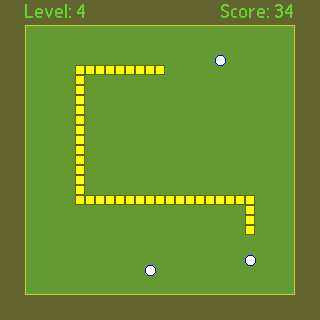
\includegraphics[scale=0.9]{./images/snake1.png}
			\end{center}
		\end{frame}
	\subsection{Requirements}
		\begin{frame}{\subsecname}
			\begin{itemize}
				\item Behavior should be consistent with \href{http://en.wikipedia.org/wiki/Snake_(video_game)}{traditional gameplay}\endnote{\href{http://www.thepcmanwebsite.com/media/flash_snake/flash_snake.shtml}{Play some Snake online} to get the hang of it}
					\begin{itemize}
						\item The game animates itself
						\item The user directs the head of the snake
						\item Colliding with goals lengthens the snake
						\item Colliding with walls or the tail ends the game
					\end{itemize}
				\item Main game controls should be the keyboard arrow keys
				\item Minimum game parameters should be set via PHP form:
					\begin{itemize}
						\item Board size
						\item Snake pace
						\item Number of simultaneous goals
					\end{itemize}
				\item Score should be tracked and displayed during play
				\item An external stylesheet should be present to skin the app
				\item There should be no javascript errors when the app runs
			\end{itemize}
		\end{frame}
	\subsection{Extra Credit Ideas}
		\begin{frame}{\subsecname}
			\begin{itemize}
				\item Implement WASD controls
					\begin{itemize}
						\item Let single players choose which set to use
						\item Allow for two concurrent players to compete
					\end{itemize}
				\item Provide additional game options accessible through the UI
					\begin{itemize}
						\item Game color scheme (snake, goals, background)
						\item Specialty board selection (e.g. - internal walls)
					\end{itemize}
				\item Implement an optional leveling system which might
					\begin{itemize}
						\item Also increase speed when goals are consumed
						\item Change the color scheme when goals are consumed
						\item Introduce timed bonus rounds where collisions don't count
					\end{itemize}
				\item Connect to a database to store high scores
				\item Validate form elements
				\item Persist form elements if validation fails
			\end{itemize}
		\end{frame}

\begin{frame}{End notes}
	\theendnotes
\end{frame}
\end{document}